\chapter{Introduction to Probability}\label{ch:intro}

\begin{quote}
{\em Life's most important questions are, for the most part, nothing but probability problems.} - Laplace
\end{quote}

In 1968 a jury found defendant Malcolm Ricardo Collins and his wife defendant Janet Louise Collins guilty of second degree robbery\cite{SULLIVAN:fk}.  The decision hinged on the testimony of bystanders, which stated that the perpetrators had been ``black male, with a beard and moustache, and a caucasian female with blonde hair tied in a ponytail,'' and that they escaped in a ``yellow motor car.''  A mathematician testified that the odds {\em against} this couple being innocent were one in {\em twelve million}, and this was enough for the jury to convict.  Later, in an appeal, the California Supreme Court reversed the decision primarily because of lack of evidence, and faulty inference.  

In another case, Sally Clark was convicted in 1999 of the murder of her two young sons\cite{KAY:2003uq}. Again, the testimony hinged on a statistical argument - the chances of one baby dying in their bed 1 in 8500, so therefore the chances of {\em two} of them dying in the same way is the square of this, or 1 in 73 million.  Several years later, and a public statement from the Royal Statistical Society highlighting the erroneous logic, Sally Clark was released - although she never overcame the resulting damage to her life that the conviction had caused.

We will cover these cases in more detail later, and why the inference was faulty, but I introduce the stories here for two reasons.  First, is to point out that there are cases in which proper statistical inference can be a life and death matter.  Second, it is to highlight the fact that such inference can run counter to one's intuition.  Part of the purpose of this book is to retrain your intuitions and your habits of intuition to avoid such failures.

We have to make decisions nearly every second of our lives, and those decisions are based on our state of knowledge.  Unfortunately, we are never 100\% sure of {\em any} information in our lives, so we are constantly forced to make decisions in the face of uncertainty.  In many cases our common sense is enough to make sophisticated decisions, taking into account the uncertain nature of the situation.  However, there are many times where our common sense is not enough to quantitatively resolve the level of uncertainty, and make valid inferences.  It is in these cases that statistical inference is most useful.  

Statistical inference refers to a field of study where we try to infer unknown properties of the world, given our observed data, in the face of uncertainty.  It is a mathematical framework to quantify what our common sense says in many situations, but allows us to exceed our common sense in cases where common sense is not enough.  Ignorance of proper statistical inference leads to poor decisions and wasted money.  As with ignorance in any other field, ignorance of statistical inference can also allow others to manipulate you, convincing you of the truth of something that is false.

For example, in 1978 a Russian satellite deviated from its orbit and became increasingly erratic, and was going to crash into the Earth.\cite{Heaps:1978qy}  This sort of event occurs from time to time, even including a recent crash of a US spy satellite in 2008.\cite{Oberg:2008fj}  There was a local news broadcast about the impending Russian satellite crash which said something like, ``the scientists had studied the trajectory of the satellite, and determined that there was only a 25\% chance of it striking land, and even a much smaller chance striking a populated area.''  The report was clearly designed to calm the public, and convince them that the scientists had a good handle on the situation.  Unfortunately, given a little thought, one realizes that the Earth's surface consists of about 25\% land and 75\% water, so {\em if you knew nothing about the trajectory of the satellite}, you would simply state that it had a 25\% chance of striking land.  Instead of communicating knowledge of the situation, the news broadcast communicated (to those who knew basic statistical inference) that either the scientists were in \emph{complete ignorance} of the trajectory or the reporter had misinterpreted a casual statement about probabilities and didn't realize what was implied.  Either way, the intent of the message and the content of the message (to those who understood basic probability) were in direct conflict.

\section{Models and Data}

There are two main aspects of statistical inference: description of data and model analysis.  In the description of data, one attempts to summarize a set of data with a smaller set of numbers.  Grades in the classroom are summarized by the average, votes in a state are summarized by a percentage, etc...  This smaller description of the data is useful for both practical and theoretical reasons.  It is more expedient to communicate a small set of numbers than the entire data set, and it is almost always the case that the detailed properties of a set of data are not relevant to the questions that you are asking.

A model refers to a mathematical structure which is used to approximate the underlying causes of the data, and unify seemingly unrelated problems.  One may have a (mathematical) model for a coin flip which ignores all of the details of the flip, the bounce, and the catch and summarizes the possible results by a single number: the chance that the coin will come up heads.  You may then use that same model to describe the voting behavior of citizens during a presidential election, or to describe the radioactive decay of particles in a physics experiment.  The mathematics is identical, but the interpretation of the components of the model will be different depending on the problem.  Models {\em simplify}, by summarizing data with a small set of causes, and they are used for {\em inference}, allowing one to predict the outcome of subsequent events.  

The goal of statistical inference is then to take data, and update our knowledge about various possible models that can describe the data.  This often means deciding which of several models is the most likely.  It can also entail the refinement of a single model, given the new data.  All of these activities are closely related to (and perhaps identical to) the methods in science.  What we are trying to do is make the best inferences from the data, improve our inferences as new data come in, and plan what data would be the most useful to improve our inferences.  In a nutshell, the approach is:

\cc{Initial Inference + New Data $\rightarrow$ Improved Inference}

In order to deal with a wide variety of problems, we require a minimal amount of mathematical structure and notation, which we introduce in this chapter.

\section{What is Probability?}

\begin{quote}
{\em Probability theory is nothing but common sense reduced to calculation.} - Laplace
\end{quote}

When you think about probability, the first things that might come to mind are coin flips (``there's a 50-50 chance of landing heads''), weather reports (``there's a 20\% chance of rain today''), and political polls (``the incumbent candidate is leading the challenger 53\% to 47\%'').  When we speak about probability, we speak about a percentage chance (0\%-100\%) for something to happen, although we often write the percentage as a decimal number, between 0 and 1.  If the  probability of an event is 0 then it is the same as saying that {\em you are certain that the event will never happen}.  If the probability is 1 then {\em you are certain that it {\em will} happen}.  Life is full of uncertainty, so we assign a number somewhere between 0 and 1 to describe our state of knowledge of the certainty of an event. The probability that you will get struck by lightning sometime in your life is $p=0.0002$, or 1 out of 5000. Statistical inference is simply the inference in the presence of uncertainty.  We try to make the best decisions we can, given incomplete information.  

\marginnote{In this book, our approach is to determine, for each problem, what degree of confidence we have in all of the possible outcomes.  
The approach of statistical inference covered in this book is about the
procedure of most rationally assigning various
degrees of confidence (which we call {\em probability}) to the possible outcomes of some process using all the objectively available data.  
}

One can think of probability as a mathematical short-hand for the common sense statements we make in the presence of uncertainty.  This short-hand, however, becomes a very powerful tool when our common sense is not up to the task of handling the complexity of a problem.  Thus, we will start with examples that will perhaps seem simple and obvious, and move to examples where it would be a challenge for you to determine the answer without the power of statistical inference.

Let's walk through a simple set of examples to establish the notation, and some of the basic mathematical properties of probabilities.

\subsection{Card Game}

A simple game can be used to explore all of the facets of probability.  We use a standard set of cards (Figure~\ref{fig:std_cards}) as the starting point, and use this system to set up the intuition, as well as the mathematical notation and structure for approaching probability problems.  

\begin{figure}
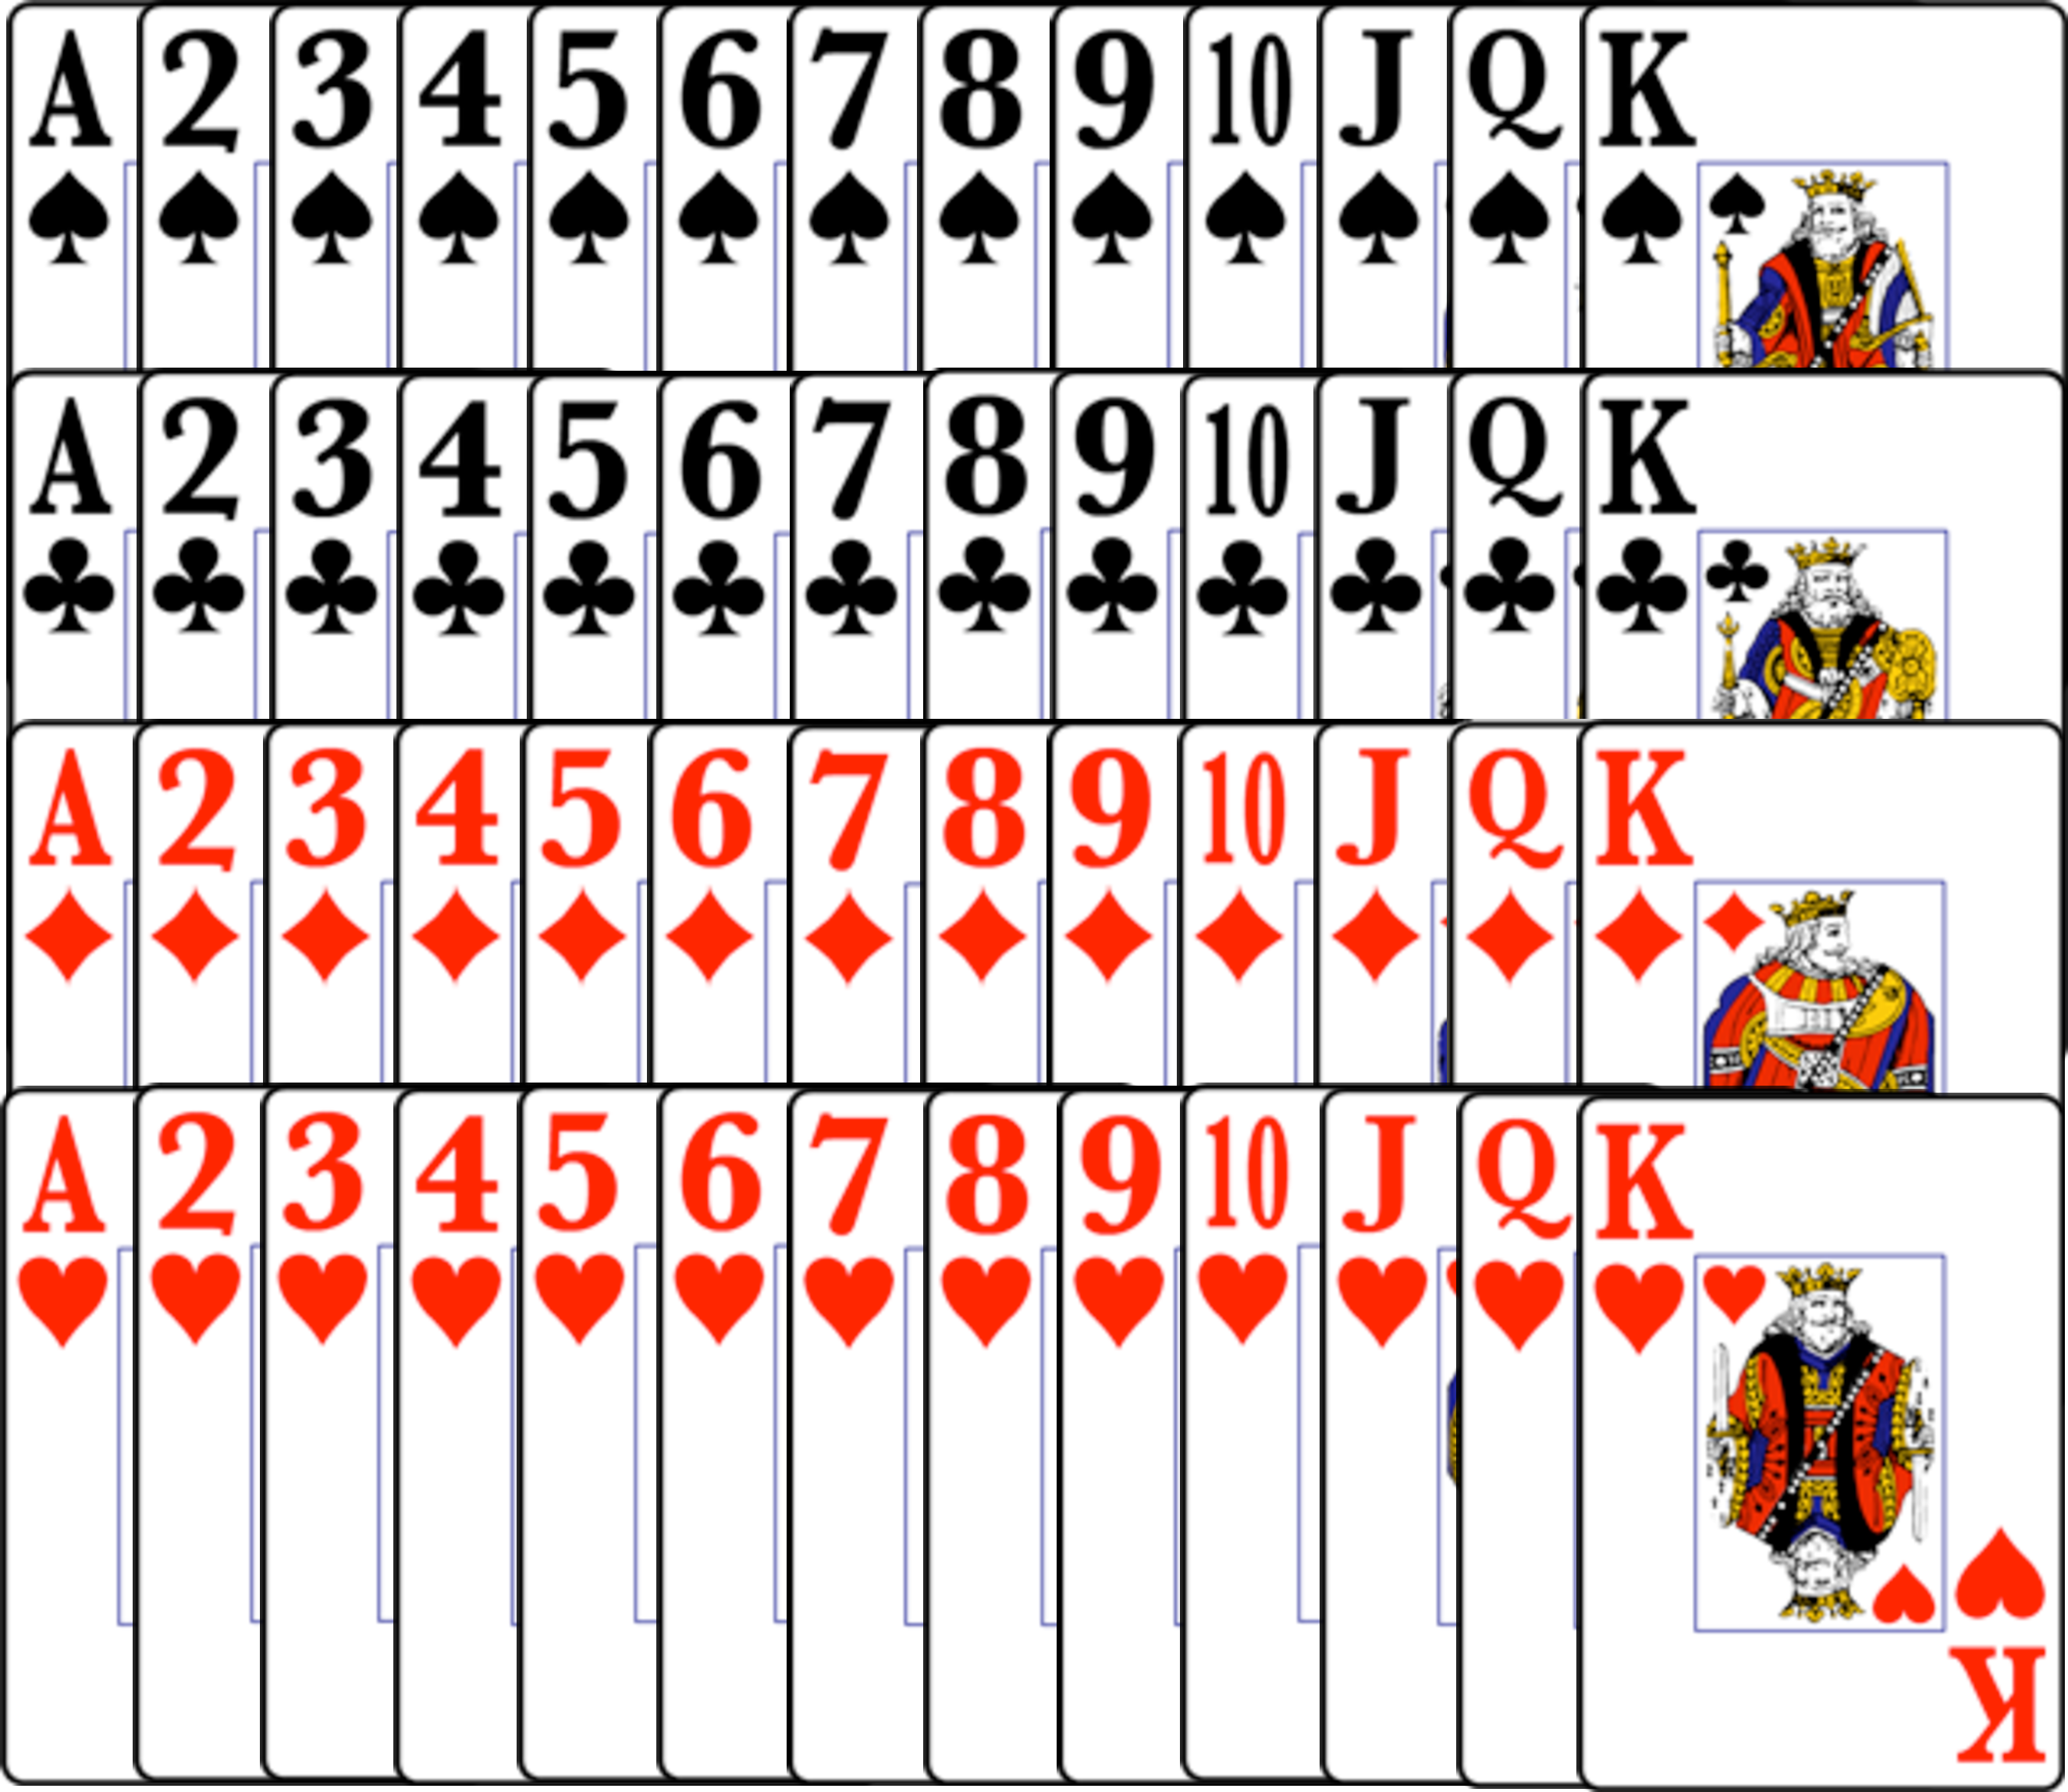
\includegraphics{StandardDeck}
\caption{Standard 52-card deck.  13 cards of each suit, labeled Spades, Clubs, Diamonds, Hearts.}\label{fig:std_cards}
\end{figure}

We start with what I simply call the {\em simple card game}\footnote{In this description of the game, we do not reshuffle after each draw.  The differences between this non-reshuffled version and the one with reshuffling will be explored later, but will only change some small details in the outcomes.}, which goes like:
\beq
\prop{simple card game}{From a standard initially shuffled deck, we draw one card, note what card it is and set it aside.  We then draw another card, note what card it is and set it aside.  Continue until there are no more cards, noting each one along the way.}
\label{eq:simplecardgame}
\eeq

There are certain principles that guide us in developing the mathematical structure of probability.  We start with some common sense notions, written in English, and then write them as general principles.  These principles, then, constrain our mathematics so that we can apply the ideas {\em quantitatively}.

When asked ``what is the probability of drawing a red on the first draw?'' you would generally say 50-50, or 50\%, or equivalently written as a probability, $P(R_{1})=0.5$. The reason for this is that we are completely ignorant of the initial conditions of the deck (i.e. where each card is located in the deck after the initial shuffling).  Given this level of (or lack of) knowledge, we could swap the colors of the two suits and we would have an equivalent state of knowledge - the problem would be identical.  We will keep coming back to this concept, but in general:
\highlight{Principle of Knowledge and Probability}{Equivalent states of knowledge must yield equivalent probability assignments.}{Equivalent states of knowledge must yield equivalent probability assignments.}

Because of this principle, we are led to the conclusion that
\beqn
P(R_{1})=P(B_{1})
\eeqn
where $R_{1}$ represents the statement ``a red on the first draw'' and $B_{1}$ represents ``a black on the first draw.''  Because these are the only two options, and they are mutually exclusive, then they must add up to 1.  Thus we have
\beqn
P(R_{1})=1-P(B_{1})
\eeqn

which leads directly to our original assignment

\beqn
P(R_{1})=P(B_{1})=0.5
\eeqn

\highlight{Mutually Exclusive}{If I have a list of {\em mutually exclusive} events, then that means that only one of them could possibly be true.  Example events include flipping heads or tails with a coins, rolling a 1, 2, 3, 4, 5 or 6 on dice, or drawing a red or black card from a deck of cards.  In terms of probability, this means that, for events A and B,  $P(A \mbox{ \bf and } B)=0$.
}{If I have a list of {\em mutually exclusive} events, then that means that only one of them could possibly be true.  Examples includes the heads and tails outcomes of coins, or the values of standard 6-sided dice.  In terms of probability, this means that, for events A and B,  $P(A \mbox{ \bf and } B)=0$.}

\highlight{Non Mutually Exclusive}{If I have a list of events that are {\em not mutually exclusive}, then it is possible for two or more to be true.  Examples include weather with rain and clouds or holding the high and the low card in a poker game.}{If I have a list of events that are {\em not mutually exclusive}, then it is possible for two or more to be true.  Examples include weather with rain and clouds or holding the high and the low card in a poker game.}

Now, this was a long-winded way to get to the answer we knew from the start, but that is how it must begin.  We start working things out where our common sense is strong, so that we know we are proceeding correctly.  We can then, confidently, apply the tools in places where our common sense is not strong.

In summary, with no more information than that there are two mutually exclusive possibilities, we assign equal probability to both.  If there are only two colors of cards in equal amounts, red and black, then the probability of drawing a red is $P(R_{1})=0.5$ and the probability for a black is the same, $P(B_{1})=0.5$.

\subsection{Other Observations}

If instead of just the color, we were interested in the suit (hearts, diamonds, spades, and clubs), then there would be four equal and mutually exclusive possibilities.  We have a certain number of possibilities, and our state of knowledge is exactly the same if we simply swap around the labels on the cards.  If we're interested in the specific card, not just the suit, the logic is the same.  Thus, we have

\beqn
P(\spades)=P(\clubs)=P(\diamonds)=P(\hearts)
\eeqn
and for drawing one specific card from the deck,
\beqn
P(A\spades)=P(2\spades)=P(3\spades)=\cdots=P(K\hearts)
\eeqn

Further, they all must add up to 1, so we get for suits
\beqn
P(\spades)+P(\clubs)+P(\diamonds)+P(\hearts)=1
\eeqn
and for the specific card from the deck,
\beqn
\underbrace{P(A\spades)+P(2\spades)+P(3\spades)+\cdots+P(K\hearts)}_{\mbox{52 cards}}=1
\eeqn

Putting it together, we get for the suits
\beqn
P(\spades)=P(\clubs)=P(\diamonds)=P(\hearts)=\frac{1}{4}
\eeqn
and for the specific card
\beqn
P(A\spades)=P(2\spades)=P(3\spades)=\cdots=P(K\hearts)=\frac{1}{52}
\eeqn

\highlight{Probabilities for Mutually Exclusive Events}{
In general, for mutually exclusive events, we have

\beq
P(A) = \frac{\mbox{(number of cases favorable to A)}}{\mbox{(total
number of equally possible cases)}}
\label{eq:p_mutually_exclusive}
\eeq
}{
\beqn
P(A) = \frac{\mbox{(number of cases favorable to A)}}{\mbox{(total
number of equally possible cases)}}
\eeqn
}


\section{Conditional Probability}

It is important to understand that probability reflects our state of knowledge about the 
system.  As our knowledge changes, so do our probability assignments.  As we gain more 
information, we change our probability assignments.  Two people observing the same 
system, but with {\em different} information about the system, will give {\em different} 
probability assignments.  All we need to make sure probability theory matches our common 
sense is for two people with the same state of knowledge, or the same information, to yield identical probability assignments.

Because our information about a system is so important in assigning probabilities, we introduce a way of writing it mathematically that we will use for the rest of the book.  It will be good for the reader to get used to reading the mathematical short-hand in English in order to gain an understanding for what it means.  



\subsection{Probability Notation}

In math, we choose to abbreviate long sentences in English, in order to use the economy of symbols.  In this book we choose a middle-ground between mathematical succinctness and the ease of understanding English.  We start with the simple card game (Equation~\ref{eq:simplecardgame})

We then define a new symbol, $|$, which should be read as ``given.''  When there is information given we call this probability {\em conditional} on that information.  When we write the following:

\beq
P(\mbox{red on first draw}|\mbox{simple card game})
\label{eq:card1}
\eeq
or
\beq
P(R_{1}|\mbox{simple card game})
\label{eq:card1a}
\eeq

this is short for 

\begin{quote}{\it ``The probability of drawing a red on the first draw, {\bf given that} we have a standard initially shuffled deck and we follow the procedure where we draw one card, note what color it is and set it aside and continue drawing, noting, and setting aside until there are no more cards.''}
\end{quote}

One can easily see that the mathematical notation is far more efficient. It is important to be able to read the notation, because it describes what we know and what we want to know.  

\highlight{Conditional Probability}{When information is given, and expressed on the right-hand side of the $|$ sign, we say that the probability is {\em conditional}.  $\Pg{I'm going to get wet today}{raining outside}$ is an assessment of how likely it is that I will get wet {\em given}, or {\em conditional on}, the fact that it is raining outside.  Clearly this number will be different if it was conditional on the fact that it is sunny outside - different states of knowledge yield different probability assignments.}{When information is given, and expressed on the right-hand side of the $|$ sign, we say that the probability is {\em conditional}.  $P($I'm going to get wet today$|$raining outside$)$ is an assessment of how likely it is that I will get wet {\em given}, or {\em conditional on}, the fact that it is raining outside.  Clearly this number will be different if it was conditional on the fact that it is sunny outside.}

\marginnote{{\em Causation}.
Imagine we have a 2-card game: a small deck with one red card and one black card, and I draw a red card first.  Clearly this makes the probability of drawing red as the second card equal to zero - it can't happen.  We're tempted to interpret 
\beqn
P(R_{2}|R_{1},\mbox{2-card game})=0
\eeqn
to mean that {\em because we drew a red on the first draw, this {\bf causes} the impossibility of drawing the red on the second} - there is only 1 red card after all, and drawing it seems to \textbf{cause} the impossibility of drawing red in the future. However, consider the following:
\beqn
P(R_{1}|R_{2},\mbox{2-card game})=0
\eeqn
which is, if we \emph{knew} that the second card we drew was red, then it makes it impossible to have drawn a red card as the first card.  This is just as true as the previous case, however, you can't interpret this as {\em causation} - the second draw didn't {\em cause} the first draw.

Instead, {\em probability statements are statements of logic, not causation}.  One can use probabilities to describe causation (i.e. $\Pg{rain}{clouds}$), but the statements of probability have no time component - later draws from the deck of cards act exactly the same as earlier ones. 
}
\comment{page 322 of Jaynes on cards and experiments}



When we put a comma (``,'') on the right side then we read this as ``and we know that.''  For example, when we write the following:


\beq
P(\mbox{red on second draw}|\mbox{simple card game,red on first draw})
\label{eq:card2}
\eeq
or
\beq
P(R_{2}|\mbox{simple card game},R_{1})
\label{eq:card2a}
\eeq

this is short for 

\begin{quote}{\it ``The probability of drawing a red on the second draw, {\bf given that} we have a standard initially shuffled deck and we follow the procedure where we draw one card, note what color it is and set it aside and continue drawing, noting, and setting aside until there are no more cards {\bf and we know} that we drew a red on the first draw.''}
\end{quote}

\section{Rules of Probability}

From the rule for mutually exclusive events (Equation~\ref{eq:p_mutually_exclusive}), we assign the following probabilities for the {\em first draw} from this deck\footnote{A face card is defined to be a Jack, Queen, or King. A number card is defined to be Ace (i.e. 1) through 10.}:
\bi
\i $P(\mbox{10})=\frac{4}{52}$
\i $P(\hearts)=\frac{13}{52}=\frac{1}{4}$
\i $P(10\hearts)=\frac{1}{52}$
\i $P(\mbox{face card})=\frac{12}{52}$ 
\i $P(\mbox{number card})=\frac{40}{52}$
\ei


It turns out that mathematically, the rules for {\em fractions of things} and of {\em probabilities} are the same.  Thus, to gain an understanding for the rules of probability, we will calculate fractions (which are more immediately intuitive), and then summarize the same rule for probabilities. 

\subsection{Negation Rule}
In this section I'll use the letter $F$ for fraction, and we can determine the values simply by counting.  The fraction of cards which are hearts ($\hearts$) is
\marginnote{{\em Either-or fallacy}. The negation rule, should not be taken to imply that everything is ``black and white,'' or ``there are only two sides to every story.''  It really is just a statement of logic, should be carefully considered and has some limitations.  For example, the following is true, 
\beqn
\P{object is black} + \P{object is not black} = 1
\eeqn
However, this does not mean the same thing as 
\beqn
\P{object is black} + \P{object is white} \neq 1
\eeqn
``Not black'' is not the equivalent of ``white.''  It could be red, or gray, or some other color.  A common logical fallacy sometimes referred to as the ``either-or fallacy'' or the ``fallacy of the excluded middle,'' turns on this point.  Some examples of these fallacies are:
\bi
\i If we don't reduce public spending, our economy will collapse.
\i You're either with us or you're a terrorist.
\i Either modern medicine can explain how Ms. X was cured, or it is a miracle.
\ei
}


\beqn
F(\hearts)=\frac{13}{52}=\frac{1}{4}
\eeqn
The fraction of cards which are {\em not} hearts (i.e. the 3 other suits) is:
\beqn
F(\mbox{not } \hearts)=\frac{13\times 3}{52}=\frac{3}{4}
\eeqn
These numbers add up to one: $F(\hearts) + F(\mbox{not } \hearts)=1$.  We can do this with more complex statements.
\beqn
\F{first card is a face card}&=&\frac{12}{52}  \\
\F{first card is not a face card}&=&\frac{40}{52} \\
\F{first card is a face card}+\F{first card is not a face card}&=&1
\eeqn

\example{What is the fraction of the first card as a jack given that we know that the first card is a face card?}

We can also apply the negation rule to conditional statements, like ``the first card is a jack given that we know that the first card is a face card.''  Notice that there are 12 cards that are face cards, so we restrict our counts to those.
\beqn
\Fg{jack}{face card}&=&\frac{4}{12} = 1/3 \\
\Fg{not a jack}{face card}&=&\frac{8}{12} = 2/3 \\
\Fg{jack}{face card}+\Fg{not a jack}{face card}&=&1
\eeqn
and they add up to one.

\highlight{Negation Rule}{
Given any information, we have
\beqn
P(\mbox{\it statement}|\mbox{\it information})+P(\mbox{{\bf not} \it statement}|\mbox{\it information})=1
\eeqn
or
\beq
P(A|B)+P(\mbox{{\bf not} } A|B)=1
\label{eq:negation}
\eeq

}{
\beqn
P(A|B)+P(\mbox{{\bf not} } A|B)=1
\eeqn
}



\subsection{Product Rule}\label{sec:product_rule}

The product rule comes from looking at the combination of events: event A {\em and} event B.  As before, we'll work on the numbers from the fractions of the card game.  

\example{What is the fraction of cards that are Jacks and a heart?}

This is clearly $\F{J$\hearts$}=1/52$, but we can look at it a different way that is equivalent.  We note that the Jacks constitute 4/52 of the cards, and that {\em of those 4}, only one quarter of them are hearts (one card out of the four cards).  So, we can arrive at the fraction of J$\hearts$ by taking one quarter of the fraction of jacks.  So what we have is
\beqn
\F{jack {\bf and} $\hearts$} = \Fg{$\hearts$}{jack}\times \F{jack}=\frac{1}{4}\times \frac{4}{52} = \frac{1}{52}
\eeqn
One can equivalently reason from the suit first: the hearts constitute 13/52 of the cards, and that {\em of those 13}, the Jacks constitute 1/13 of the cards.  So, we can arrive at the fraction of J$\hearts$ by taking one thirteenth of the fraction of $\hearts$.  Again, we have

\beqn
\F{jack {\bf and} $\hearts$} = \Fg{jack}{$\hearts$}\times \F{$\hearts$}=\frac{1}{13}\times \frac{13}{52} = \frac{1}{52}
\eeqn
In general we have 
\highlight{Product Rule}{
\beq
P(A\mbox{ and }B)=P(A|B)P(B)= P(B|A)P(A) \label{eq:product}
\eeq
}{
\beqn
P(A\mbox{ and }B)&=&P(A|B)P(B)\\
&=& P(B|A)P(A) 
\eeqn
}
\example{What is the probability of drawing two Kings in a row?}
 This is the same as
\beqn
P(K_{2}\mbox{ and }K_{1})
\eeqn
From the product rule (Equation~\ref{eq:product}) we have
\beqn
P(K_{2}\mbox{ and }K_{1})&=&P(K_{2}|K_{1})P(K_{1})
\eeqn
The second part is straight forward: $P(K_{1})=4/52$.  The first part is asking the probability of drawing a second king, knowing that we have drawn a king on the first draw.  Now, there are only 51 cards remaining when we do the second draw, and only 3 kings.  Thus, we have $P(K_{2}|K_{1})=3/51$ and finally
\beqn
P(K_{2}\mbox{ and }K_{1})&=&P(K_{2}|K_{1})P(K_{1}) \\
&=&\frac{3}{51}\times \frac{4}{52} = \frac{1}{221}
\eeqn




\subsection{Independence}\label{sec:independence}

As a specific case of the product rule, we can change the rule of the card games such that we reshuffle the deck after each draw.  In this way, the result of one draw gives you no information about other draws.  In this case, the events are considered {\em independent}. 

\highlight{Independent Events}{Two events, A and B, are said to be independent if knowledge of one gives you no information on the other. Mathematically, this means
\beqn
P(A|B)=P(A)
\eeqn
and
\beqn
P(B|A)=P(B)
\eeqn
}{Two events, A and B, are said to be independent if knowledge of one gives you no information on the other. Mathematically, this means
\beqn
P(A|B)=P(A)
\eeqn
and
\beqn
P(B|A)=P(B)
\eeqn
}

In this  case, the product rule reduces to the simplified rule for independent events: the product of the individual event probabilities.

\highlight{Joint Probabilities for Independent Events}{
\beq
\P{$A$ {\bf and} $B$}=P(A)\times P(B)
\label{eq:indepprod}
\eeq
}{
\beqn
\P{$A$ {\bf and} $B$}=P(A)\times P(B)
\eeqn
}

We have already seen an example of this, when we looked at drawing the Jack of Hearts: drawing a heart gives you no information about whether it is a jack, and vice versa.  Thus,
\beqn
\Pg{$\hearts$}{jack} = \P{$\hearts$}
\eeqn

\example{What is the probability of flipping two heads in a row?}

The probability of getting ``heads'' on any given coin flip is $P(H)=0.5$.  The probability of flipping two heads in a row is then simply $P(H_{1}) \times P(H_{2})=0.5\times 0.5 = 0.25$, because the second flip is independent of the first.  If it wasn't, then you'd have to determine how the knowledge of the first flip influences our knowledge of the second flip, which is written as $P(H_{2}|H_{1})$ and the full product rule (Equation~\ref{eq:product}) would need to be used.

\subsection{Conjunction}\label{sec:conjunction}

One of the consequences of combinations of events is that the probability of two events happening, A {\bf and} B, has to be less than (or possibly equal to) the probability of just one of them, say A, happening.  The mathematical fact is seen by looking at the magnitude of the terms in the product rule
\beqn
\P{$A$ and $B$} = \underbrace{P(B|A)}_{\parbox{.5in}{less than or equal to 1}}\times P(A) \leq P(A)
\eeqn

In other words, coincidences are less likely than either event happening individually.  We intuitively know this, when we make comments like ``Wow! What are the chances of that?'' referring to, say, someone winning the lottery and then getting struck by a car the next day.  Sometimes, however, it seems as if one's intuition does not match the conclusions of the rules of probability.  One such case is called the {\em conjunction fallacy}.\marginnote{{\em Combinations of Events and the English language}
I believe that the issue of the conjunction fallacy is more subtle than this.  In English, if I were to say ``Do you want steak for dinner, or steak and potatoes?'' one would immediately parse this as choice between
\be
\i steak with no potatoes
\i steak with potatoes
\ee
Although strict logic would parse this choice as
\be
\i steak, possibly with potatoes and possibly without potatoes
\i steak, definitely with potatoes,
\ee
it is common in English to have the implied negative (i.e. steak with no potatoes) when given a choice where the alternative is a conjunction (i.e. steak with potatoes). }

In an interesting experiment, Tversky and Kahneman\citep{tversky1983extensional} gave the following survey:


\begin{quote}Linda is 31 years old, single, outspoken, and very bright. She majored in philosophy. As a student, she was deeply concerned with issues of discrimination and social justice, and also participated in anti-nuclear demonstrations.

Which is more probable?
\be
\i Linda is a bank teller.
\i Linda is a bank teller and is active in the feminist movement.
\ee
\end{quote}
85\% chose option 2.\citep{tversky1974judgment}  This, they attributed, to the conjunction fallacy - mistaking the conjunction of two events as more probable than a single event.  They went further and did a survey of medical internists with the following
\begin{quote}
Which is more likely: the victim of an embolism (clot in the lung) will experience partial paralysis or that the victim will experience both partial paralysis and shortness of breath?
\end{quote}\marginnote{{\em Combinations of Events and the English language} If we interpret the doctor's choice with this implied negative, we have:
\be
\i clot with paralysis and no shortness of breath
\i clot with paralysis and shortness of breath
\ee
and the first one is much less likely, because it would be odd to have a clot and not have a very common symptom associated with it.  The doctor's probability assessment is absolutely correct: both symptoms together are more likely than just one.  The ``fallacy'' arises because the English language is sloppier than mathematical language.
}

and again, 91 percent of the doctors chose that the clot was less likely to cause the rare paralysis rather than to cause the combination of the rare paralysis and the common shortness of breath.

Even when correct, the consequence for conjunctions can be misused, or at least misidentified.  Returning to our example of someone winning the lottery and then getting struck by a car the next day, rare events {\em occur frequently}, as long as you have enough events.  There are millions of people each day playing the lottery, and millions getting struck by cars each day.  We will explore this problem later in Section~\ref{sec:lottery}, but one immediate consequence is that winning the lottery and getting struck by a car the next day probably happens {\em somewhere} fairly regularly.



\subsection{Sum Rule}\label{sec:sumrule}

Now we consider the statements of the form A {\bf or} B.  For example, in the card game, what is the fraction of cards that are jacks or are hearts.  By counting we get the 13 hearts and 3 more jacks that are not contained in the 13 hearts, or $\F{jack {\bf or} $\hearts$}=\frac{13+3}{52}=16/52$.  Now, if we tried to separate the terms, and do:
\beqn
\F{jack} + \F{$\hearts$} = \frac{4}{52} + \frac{13}{52} =\frac{17}{52}
\eeqn  
then we get a number that is too big!  It is too big because we've double-counted the jack of hearts.  Adjusting for this, by subtracting one copy of this fraction, we get
\beqn
\F{jack} + \F{$\hearts$} - \F{jack {\bf and} $\hearts$}= \frac{4}{52} + \frac{13}{52} -\frac{1}{52}=\frac{16}{52} = \F{jack {\bf or} $\hearts$}
\eeqn  
In general 
\highlight{Sum Rule}{
\beq
P(A \mbox{ \bf or } B)=P(A)+P(B)-P(A \mbox{ \bf and } B)
\label{eq:sum}
\eeq
}{
\beqn
P(A \mbox{ \bf or } B)=P(A)+P(B)-P(A \mbox{ \bf and } B)
\eeqn
}

\highlight{Sum Rule for Exclusive Events}{If two events are {\em mutually exclusive} the sum rule reduces to
\beq
P(A \mbox{ \bf or } B) = P(A) + P(B)
\label{eq:exclusive_sum}
\eeq
because $P(A \mbox{ \bf and } B)=0$ for such events.

So the probability of rolling a 1 or a 2 on one die is 2/6.
}{If two events are {\em mutually exclusive} the sum rule reduces to
\beqn
P(A \mbox{ \bf or } B) = P(A) + P(B)
\eeqn
because $P(A \mbox{ \bf and } B)=0$ for such events.
}

One more variant on the Sum Rule is where we have 3 propositions.  It can be a bit tedious to write it all out, but the end result looks a lot like the original Sum Rule.  All we do is break up the terms in pieces, and then apply the Sum Rule to each piece.
\beqn
P(A \mbox{ \bf or } B \mbox{ \bf or } C) &=&P(A \mbox{ \bf or } \left[B \mbox{ \bf or } C\right]) \\
&=&P(A)+P(B \mbox{ \bf or } C)-P(A \mbox{ \bf and } \left[B \mbox{ \bf or } C\right]) \\
&=&P(A)+P(B)+P(C)-P(B \mbox{ \bf and } C) - \\
&&P(A \mbox{ \bf and } B \mbox{ \bf or } A \mbox{ \bf and } C)\\
&=&P(A)+P(B)+P(C)-P(B \mbox{ \bf and } C) - \\
&&\left[P(A \mbox{ \bf and } B)+P(A \mbox{ \bf and } C)-\right.\\
&&\left.P(A \mbox{ \bf and } B\mbox{ \bf and } A\mbox{ \bf and } C)\right]
\eeqn
which leads finally to
\highlight{Sum Rule for Three Events}{
\beq
\nn P(A \mbox{ \bf or } B \mbox{ \bf or } C) &=&P(A)+P(B)+P(C)-\\
\nn&&P(A \mbox{ \bf and } B)-P(B \mbox{ \bf and } C)-P(A \mbox{ \bf and } C)+\\
&&P(A \mbox{ \bf and } B\mbox{ \bf and } C)
\label{eq:sum3}
\eeq
}{
\beqn
P(A \mbox{ \bf or } B \mbox{ \bf or } C) &=&P(A)+P(B)+P(C)-\\
&&P(A \mbox{ \bf and } B)-\\
&&P(B \mbox{ \bf and } C)-\\
&&P(A \mbox{ \bf and } C)+\\
&&P(A \mbox{ \bf and } B\mbox{ \bf and } C)
\eeqn
}
In words, when you're looking for the sum of several events, we add the probabilities (i.e. $P(A)+P(B)+P(C)$), then subtract the double counting (i.e. $P(A \mbox{ \bf and } B)$) as before.  Finally, we need to add back in the {\em triple count} (i.e. $P(A \mbox{ \bf and } B\mbox{ \bf and } C)$) because it was taken out too many times with the double count.  The accounting here can be somewhat prone to error, but the concepts are always the same: when you add probabilities of events, say $A$ and $B$, together the term $P(A)$ includes the probability of both $P(A \mbox{ \bf and } B)$ and the term $P(B)$ includes the probability of both $P(A \mbox{ \bf and } B)$, so you've included that probability twice and need to subtract one of them to balance the books.  Likewise (although it is harder to show), the first six terms in Equation~\ref{eq:sum3} end up subtracting one too many copies of $P(A \mbox{ \bf and } B\mbox{ \bf and } C)$, and we need to add one in at the end.

\subsection{Marginalization}\label{sec:marginalization_intro}

Another consequence of the sum rule and the product rule is a process called {\em marginalization}.  

\example{Marginalization and Card Suit}
Imagine we have a number of conditional statements, like:
\beqn
\Pg{jack}{$\hearts$}&=&\frac{1}{13} \\
\Pg{jack}{$\diamonds$}&=&\frac{1}{13} \\
\Pg{jack}{$\spades$}&=&\frac{1}{13} \\
\Pg{jack}{$\clubs$}&=&\frac{1}{13}
\eeqn
but we are interested in just the probability of drawing a jack, regardless of the suit, or in our notation
\beqn
\P{jack}
\eeqn
The marginalization procedure for this problem looks like:

\beqn
\P{jack}&=& \overbrace{\Pg{jack}{$\hearts$}\times \P{$\hearts$} +}^{\mbox{all possibilities}}\\
&&\Pg{jack}{$\diamonds$}\times \P{$\diamonds$} +\\
&&\Pg{jack}{$\spades$}\times \P{$\spades$} +\\
&&\Pg{jack}{$\clubs$}\times \P{$\clubs$} \\
&=& \frac{1}{13}\times\frac{1}{4}+\frac{1}{13}\times\frac{1}{4}+\frac{1}{13}\times\frac{1}{4}+\frac{1}{13}\times\frac{1}{4} \\
&=&\frac{4}{52}
\eeqn
\newpage
\highlight{Marginalization}{If we have a complete set of conditional statements, like
\beqn
&P(A|B_{1})&\\
&P(A|B_{2})&\\ 
&P(A|B_{3})&\\
&P(A|B_{4})&\\
& \vdots&
\eeqn
then the {\em unconditional} probability is found by {\em marginalizing} over all possible values of the conditional events, like
\beq
P(A)=\overbrace{P(A|B_{1})P(B_{1})+ P(A|B_{2})P(B_{2})+ P(A|B_{3})P(B_{3})+ \cdots}^{\mbox{all possible $B$s}}
\label{eq:marginalization}
\eeq
}{If we have a complete set of conditional statements, like
\beqn
P(A|B_{1}), P(A|B_{2}), P(A|B_{3}), P(A|B_{4}), \cdots
\eeqn
then the {\em unconditional} probability is found by {\em marginalizing} over all possible values of the conditional events, like
\beqn
P(A)=\overbrace{P(A|B_{1})P(B_{1})+ P(A|B_{2})P(B_{2})+ \cdots}^{\mbox{all possible $B$s}}
\eeqn
}


\subsection{Bayes' Rule}

\marginnote{In the 1700's Reverend Bayes proved a special case of this rule, and rediscovered in the general form by Pierre-Simon Laplace.  Laplace then applied the rule in a large range of problems from geology, astronomy, medicine, and jurisprudence.}One of the most consequential rules of probability is what is known as Bayes' Rule, sometimes called Bayes' Theorem.  We will use this rule throughout this book, and see its many applications.  It comes as a direct result of the product rule (Equation~\ref{eq:product})
\beqn
P(A\mbox{ and }B)=P(A|B)P(B)= P(B|A)P(A)
\eeqn
Rearranging, we get
\highlight{Bayes' Rule}{
\beq
P(A|B) = \frac{P(B|A)P(A)}{P(B)} \label{eq:bayes}
\eeq
}{
\beqn
P(A|B) = \frac{P(B|A)P(A)}{P(B)} 
\eeqn
}

We can verify this again with the intuitions we have in the simple card game.  

\example{What is the probability of drawing a jack, knowing that you've drawn a face card?}

 In terms of fractions, this should be $\Fg{jack}{face card}=4/12=1/3$. Applying Bayes' Rule to the fractions we get:

\beqn
\Fg{jack}{face}&=&\frac{\Fg{face}{jack}\times\F{jack}}{\F{face}}\\
&=&\frac{\frac{4}{4}\times \frac{4}{52}}{\frac{12}{52}}=\frac{4}{12}=\frac{1}{3}
\eeqn
Although this calculation is true, it isn't particularly enlightening.  It is nicer to cast the problem back into probability terms, rather than fractions, and compare the probability of drawing a jack to the probability of the same thing (i.e. drawing a jack) {\em given} that we know that we've drawn a face card.  This is
\beqn
\P{jack} &=& \frac{1}{13} \\
\Pg{jack}{face card} &=& \frac{1}{3}
\eeqn

This comparison highlights what Bayes' Rule represents: learning.\marginnote{All of learning is simply updating ones beliefs given the data.  The data may be words in a book, the results of an experiment, a conversation with another person, etc...  The strength of our beliefs are not often thought of in mathematical terms, but you are doing the math of probabilities whenever you are weighing the strength of your beliefs.  Thus, the probabilistic rule - Bayes' rule - for updating beliefs given data is really the quantitative specification of learning.  One can use it \emph{qualitatively} as well, which is often useful in fields such as history where the data do not tend to be quantitative.}  When you are asked what the probability of drawing a jack, from the knowledge of the simple card game, you calculate the value of 1/13.  Once you learn that you drew a face card, you update your knowledge to include that information, and modify your probability assignments to reflect this.  This leads to an increased chance of the card being a jack.  

In a nutshell, Bayes' Rule represents learning:
\beqn
\mbox{Initial Belief} + \mbox{New Data} \rightarrow \mbox{Improved Belief}
\eeqn

It is used in science to infer causes from effects, and can thus be written
\beqn
\Pg{cause}{effect} &=& \frac{\Pg{effect}{cause}\times \P{cause}}{\P{effect}}
\eeqn
To infer the probability of a particular cause, given the events you observe in the world, you first have to know the probability of the cause itself (i.e. rarer causes will reduce the {\em prior} probability), and how likely that the cause you're looking at could have produced the effects you've observed.  These two items are the $\P{cause}$ and $\Pg{effect}{cause}$ terms, respectively.  The entire calculation is scaled by $\P{effect}$ which is {\em all of the other ways that the effects could have been produced by other causes.}.  Thus, it is not enough to show that giving a particular medicine is followed by the symptoms disappearing to establish that the medicine was the likely cause of the symptoms disappearing.  You have to calculate what other possible causes could have had those effects, such as the normal functioning of the immune system or the placebo effect.  This is why carefully controlled studies are necessary, to eliminate all of the other possible causes and to determine the true cause of the effects observed.

We will spend large portions of several chapters on Bayes' Rule, to explore its long-ranging consequences.
\newpage
\section{Venn Mnemonic for the Rules of Probability}
\begin{marginfigure}
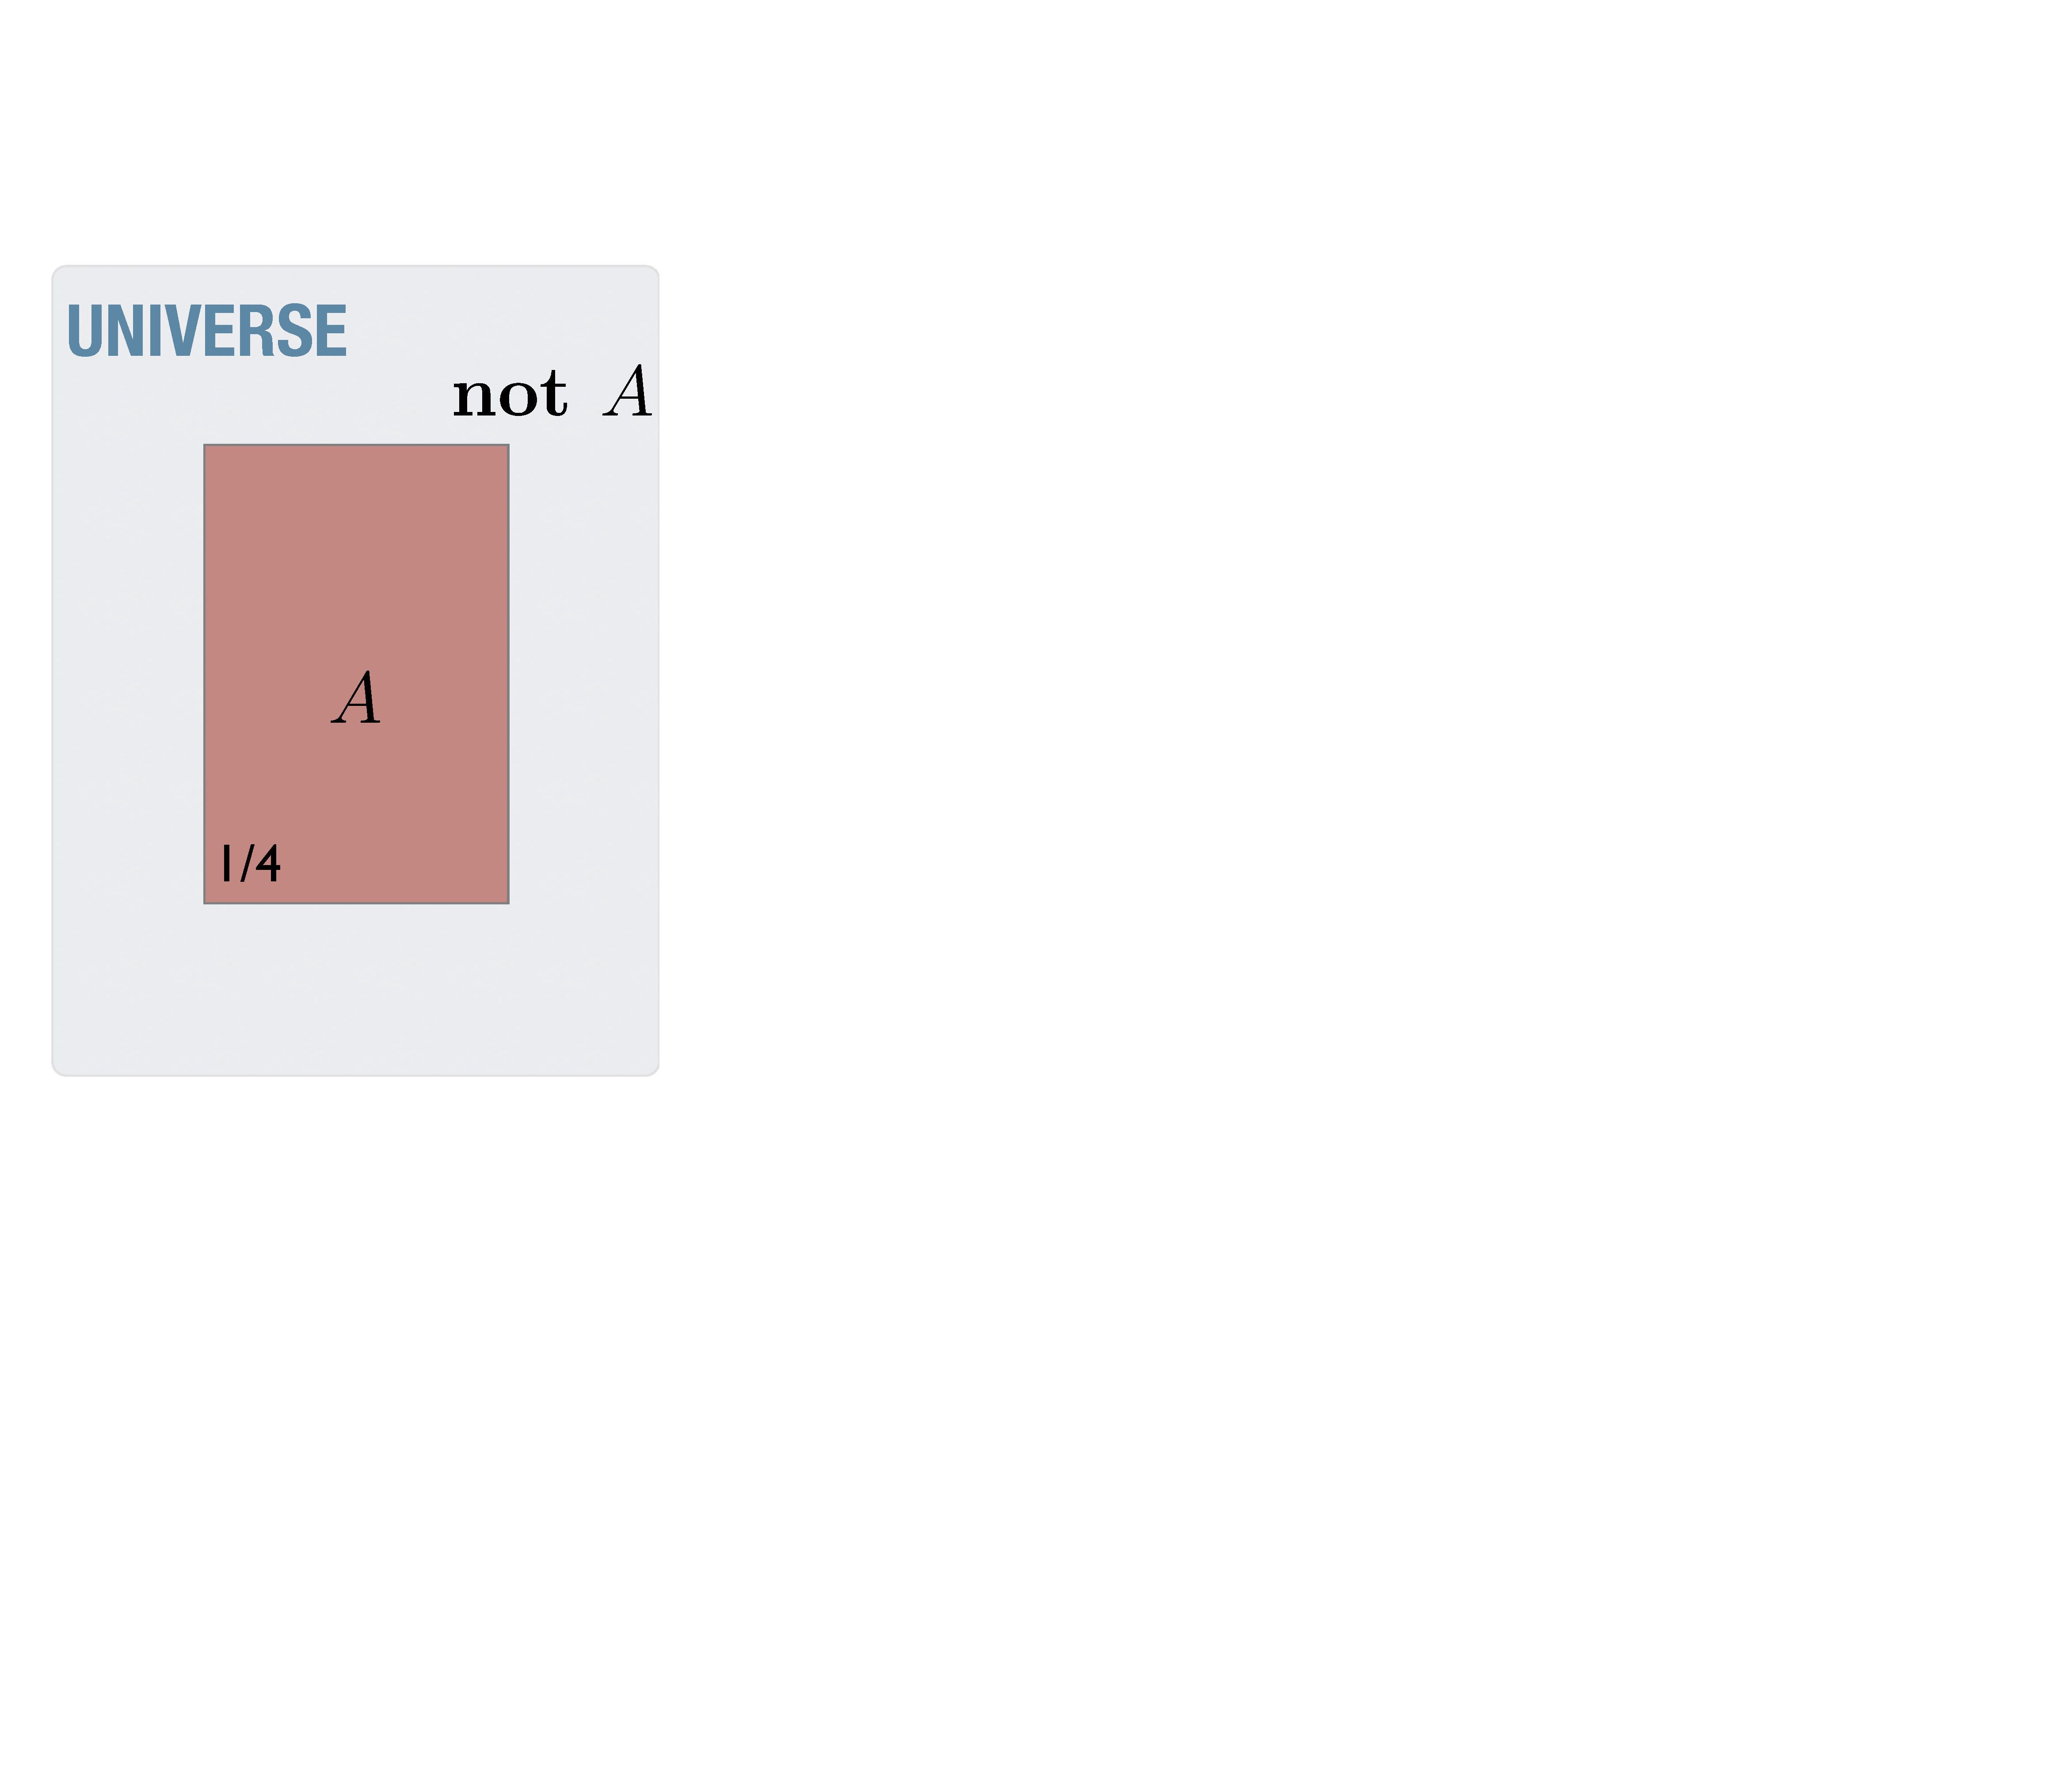
\includegraphics[width=1.4in]{venn1}
\caption{Venn diagram of a statement, $A$, in a {\em Universe} of all possible statements.  It is customary to think of the area of the {\em Universe} to be equal to 1 so that we can treat the actual areas as fractional areas representing the probability of statements like $P(A)$.  In this image, $A$ takes up 1/4 of the {\em Universe}, so that $P(A)=1/4$.  Also shown is the negation rule.  $P(A)+P(\mbox{{\bf not} } A)=1$ or ``inside'' of $A$ + ``outside'' of $A$ adds up to everything.}
\label{fig:venn_negation}
\end{marginfigure}

It is often useful to have a picture to represent the mathematics, so that it is easier to remember the equations and to understand their meaning.  It is common to use what is called a Venn Diagram to represent probabilities in an intuitive, graphical way.  The idea is that probabilities are represented as the {\em fractional area} of simple geometric shapes.  We can then find a picture representation of each of the rules of probability.  We start by looking at a sample Venn Diagram, in Figure~\ref{fig:venn_negation}.

\begin{marginfigure}
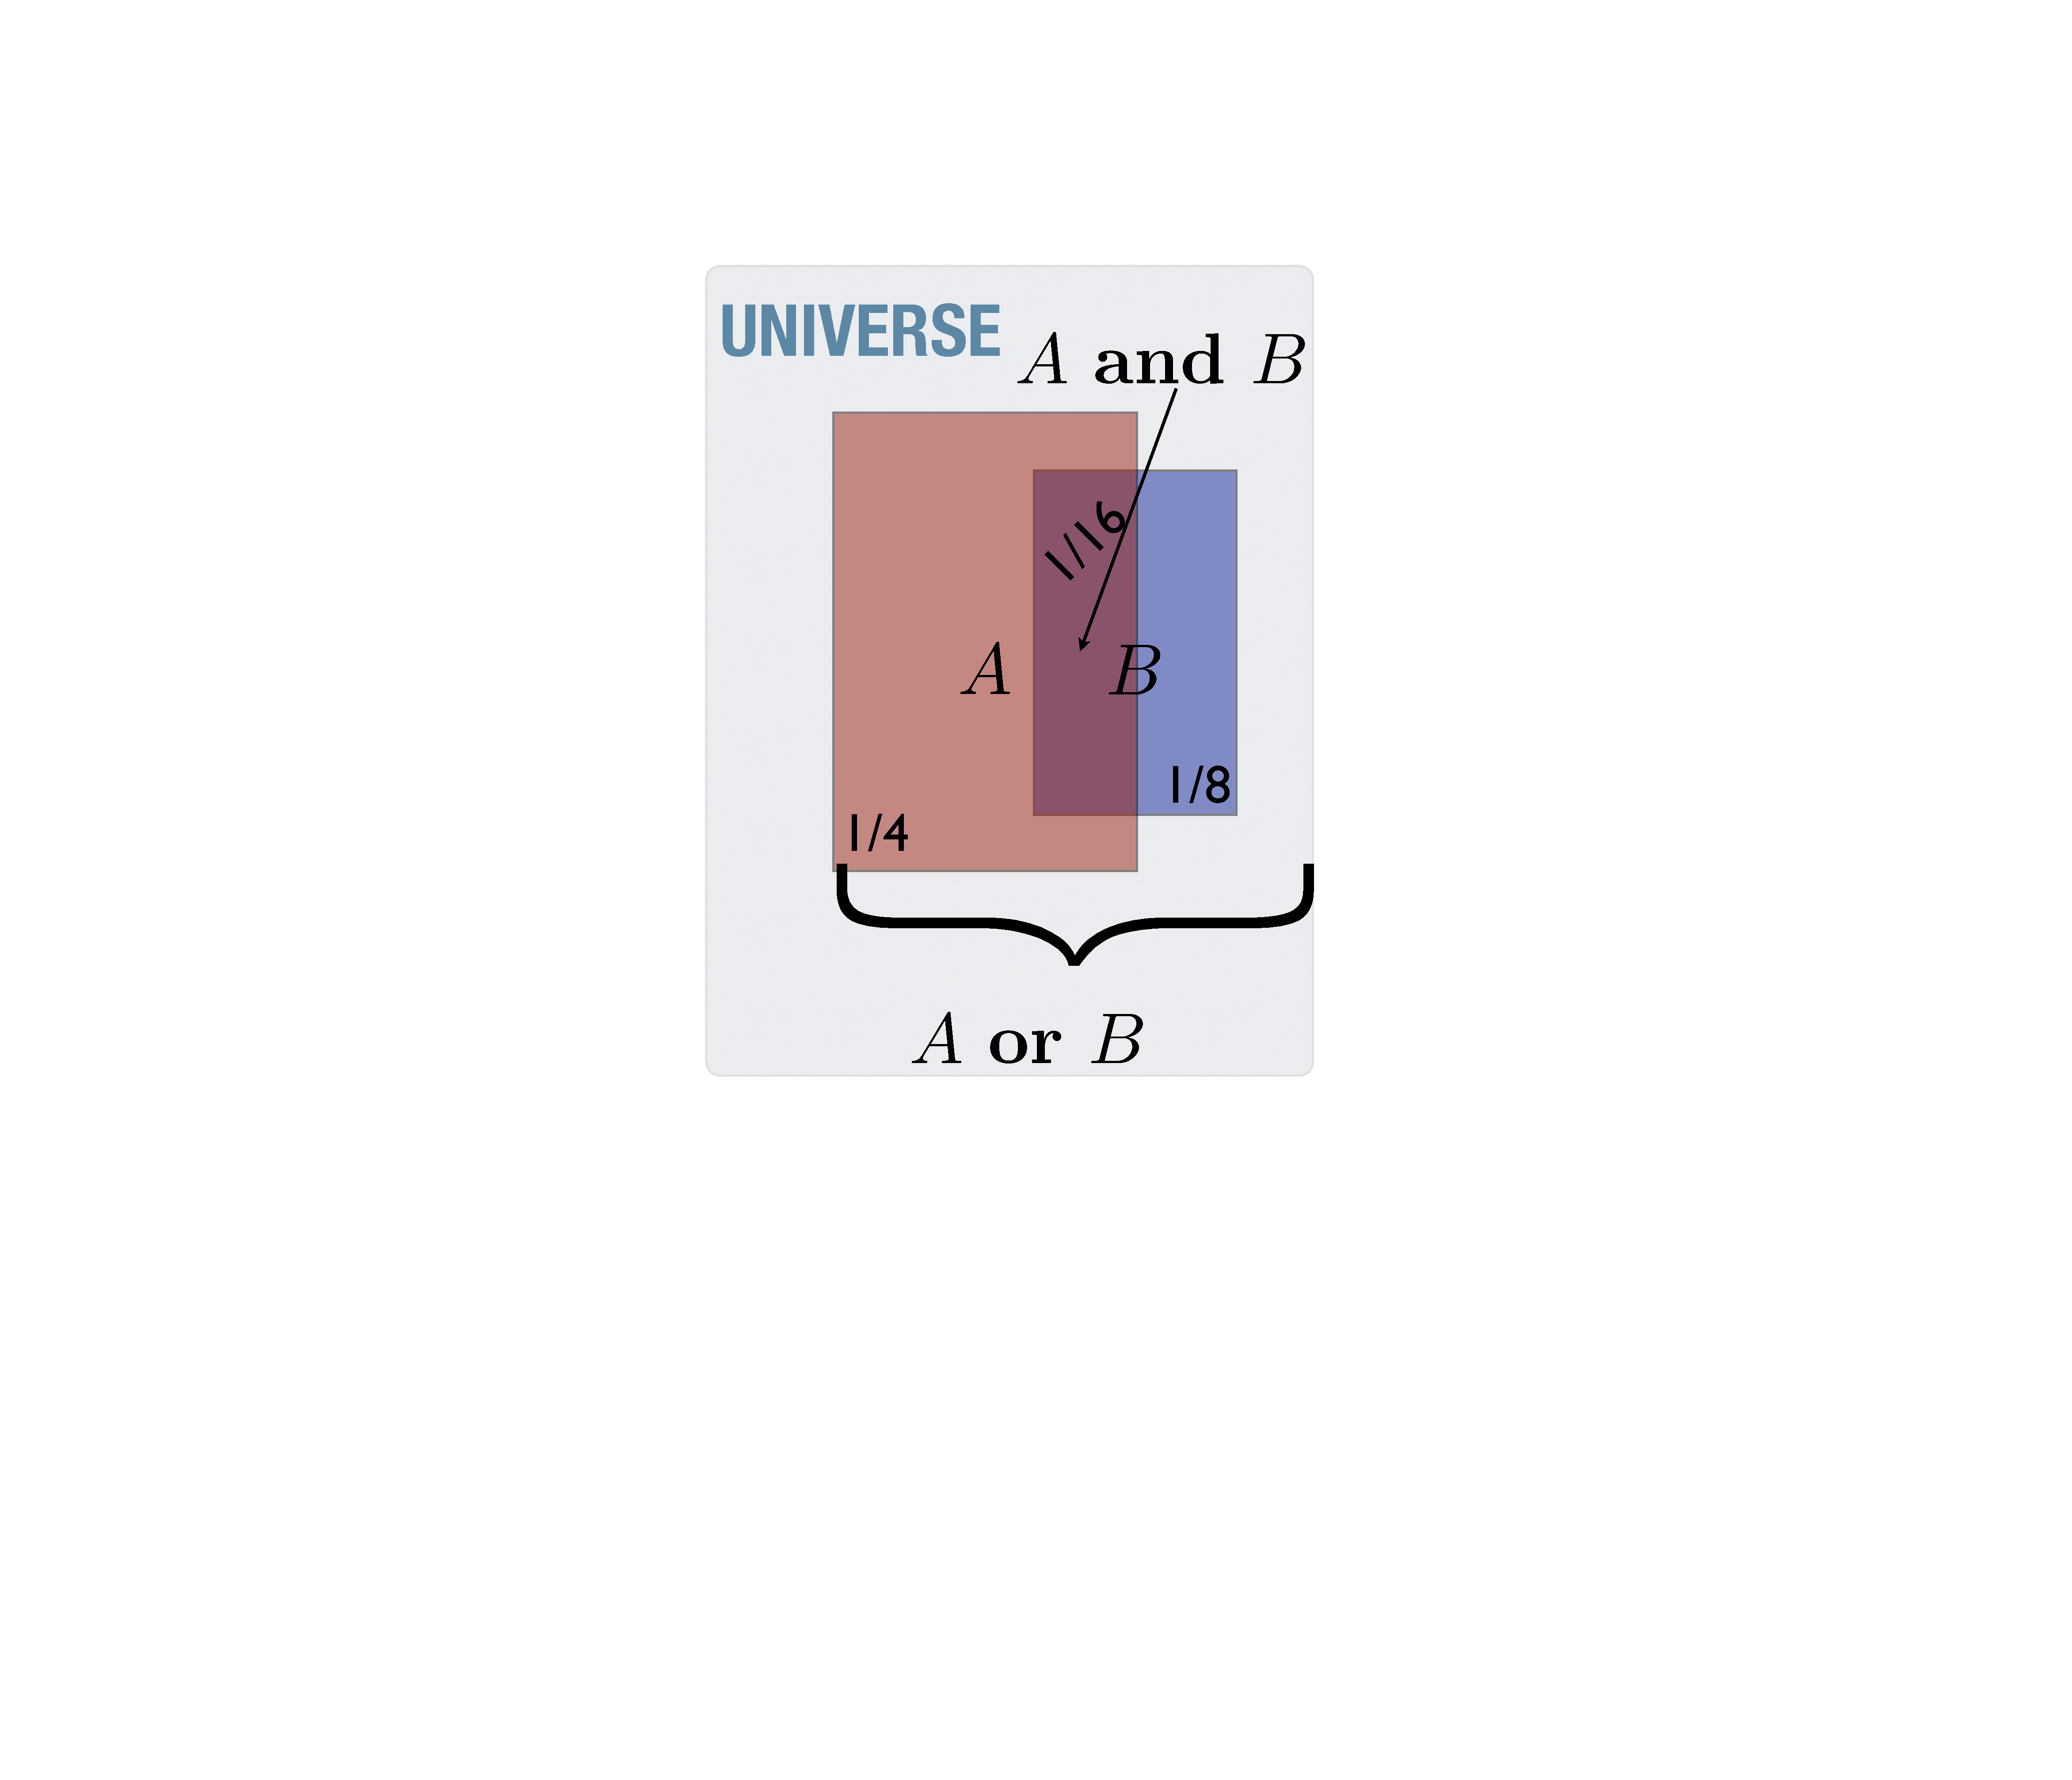
\includegraphics[width=1.4in]{venn2}
\caption{Venn diagram of the sum and product. The rectangle $B$ takes up 1/8 of the {\em Universe}, and the rectangle $A$ takes up 1/4 of the {\em Universe}.  Their overlap here is 1/16 of the {\em Universe}, and represents $P(A \mbox{ and } B)$.  Their total area of 5/16 of the {\em Universe} represents $P(A \mbox{ or } B)$.}
\label{fig:venn_and_or}
\end{marginfigure}
The fractional area of the rectangle $A$ represents the probability $P(A)$, and can be thought of as a probability of one of the statements we've explored, such as $P(\hearts)$.  This diagram is strictly a mnemonic, because the individual points on the diagram are not properly defined.  The diagram in Figure~\ref{fig:venn_negation} also represents the Negation Rule (Equation~\ref{eq:negation}),
\beqn
P(A)+P(\mbox{{\bf not} } A)=1
\eeqn
In the diagram it is easy to see that the sum of the areas inside of $A$ (i.e. 1/4) and outside of $A$ (i.e. 3/4) cover the entire area of the {\em Universe} of statements, and thus add up to 1. 

Figure~\ref{fig:venn_and_or} shows the diagram which can help us remember the sum and product rules.  The Sum Rule (Equation~\ref{eq:sum})
\beqn
P(A \mbox{ \bf or } B)=P(A)+P(B)-P(A \mbox{ \bf and } B)
\eeqn
is represented in the total area occupied by the rectangles $A$ and $B$, and makes up all of $A$ (i.e. 1/4) and the half of $B$ sticking out (i.e. 1/8-1/16=1/16) yielding $P(A \mbox{ or } B)=5/16$.  This is also the area of each added up (1/4+1/8), but subtracting the intersection (1/16) because otherwise it is counted twice.  Adding the areas this way directly parallels the Sum Rule.  

Conditional probabilities, like those that come into the Product Rule (Equation~\ref{eq:product}) and Bayes Rule (Equation~\ref{eq:bayes}) are a little more challenging to visualize.  In Figure~\ref{fig:venn_conditional}, $P(A|B)$ is represented by the fraction of the darker area (which was originally part of $A$) compared not to the {\em Universe} but to the area of $B$, and thus represents $P(A|B)=1/2$.  In a way, it is as if the conditional symbol, ``$|$,'' defines the {\em Universe} with which to make the comparisons.  On the left of Figure~\ref{fig:venn_conditional}, the same darker area that was originally part of $B$ represents $P(B|A)$ making up 1/4 of the area of $A$.  Thus $P(B|A)=1/4$.  The Product Rule (Equation~\ref{eq:product}) then follows,
\beqn
P(A\mbox{ and }B)=\underbrace{P(A|B)}_{1/2}\underbrace{P(B)}_{1/8}= \underbrace{P(B|A)}_{1/4}\underbrace{P(A)}_{1/4} = \frac{1}{16}
\eeqn

We can further see the special case of mutually exclusive statements shown in Figure~\ref{fig:venn_exclusive}. The Sum Rule for Exclusive Events (Equation~\ref{eq:exclusive_sum}) is simply the sum of the two areas because there is no overlap

\begin{marginfigure}
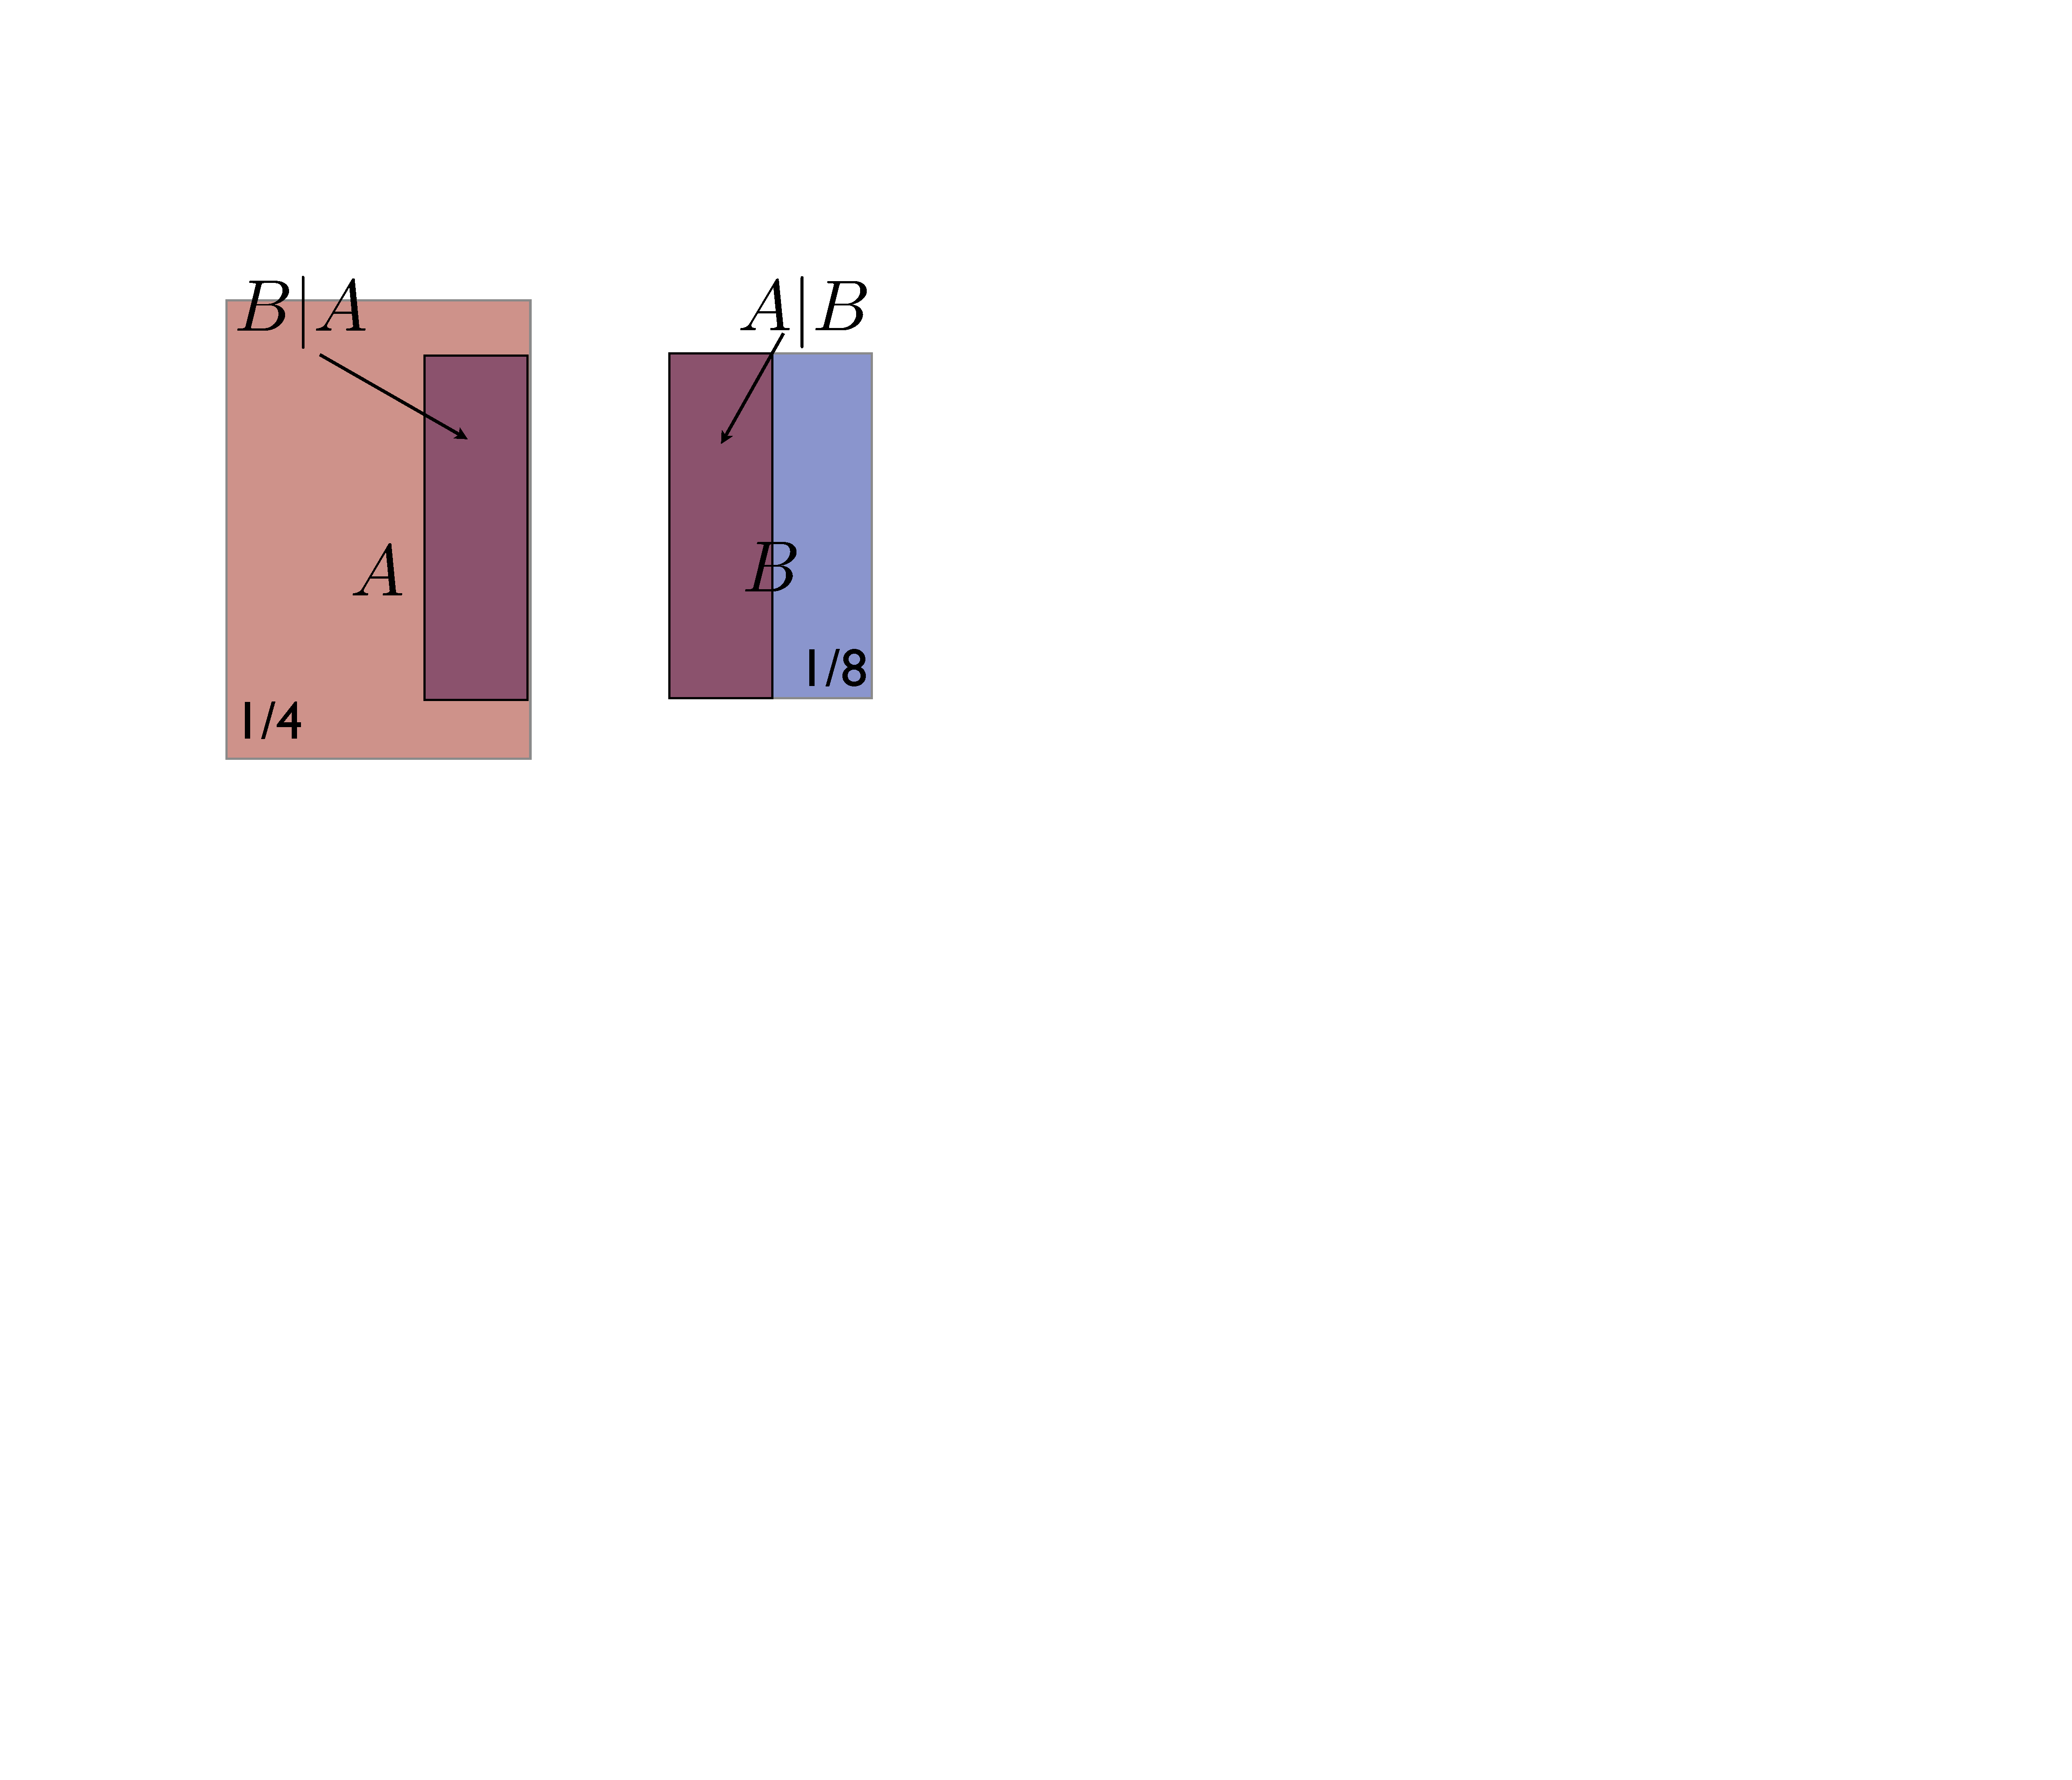
\includegraphics[width=1.4in]{venn4}
\caption{Venn diagram of conditional probabilities, $P(A|B)$ and $P(B|A)$.  (Right) $P(A|B)$ is represented by the fraction of the darker area (which was originally part of $A$) compared not to the {\em Universe} but to the area of $B$, and thus represents $P(A|B)=1/2$.  In a way, it is as if the conditional symbol, ``$|$,'' defines the {\em Universe} with which to make the comparisons.  (Left) Likewise, the same darker area that was originally part of $B$ represents $P(B|A)$ which makes up 1/4 of the area of $A$.  Thus $P(B|A)=1/4$.  }
\label{fig:venn_conditional}
\end{marginfigure}


\begin{marginfigure}
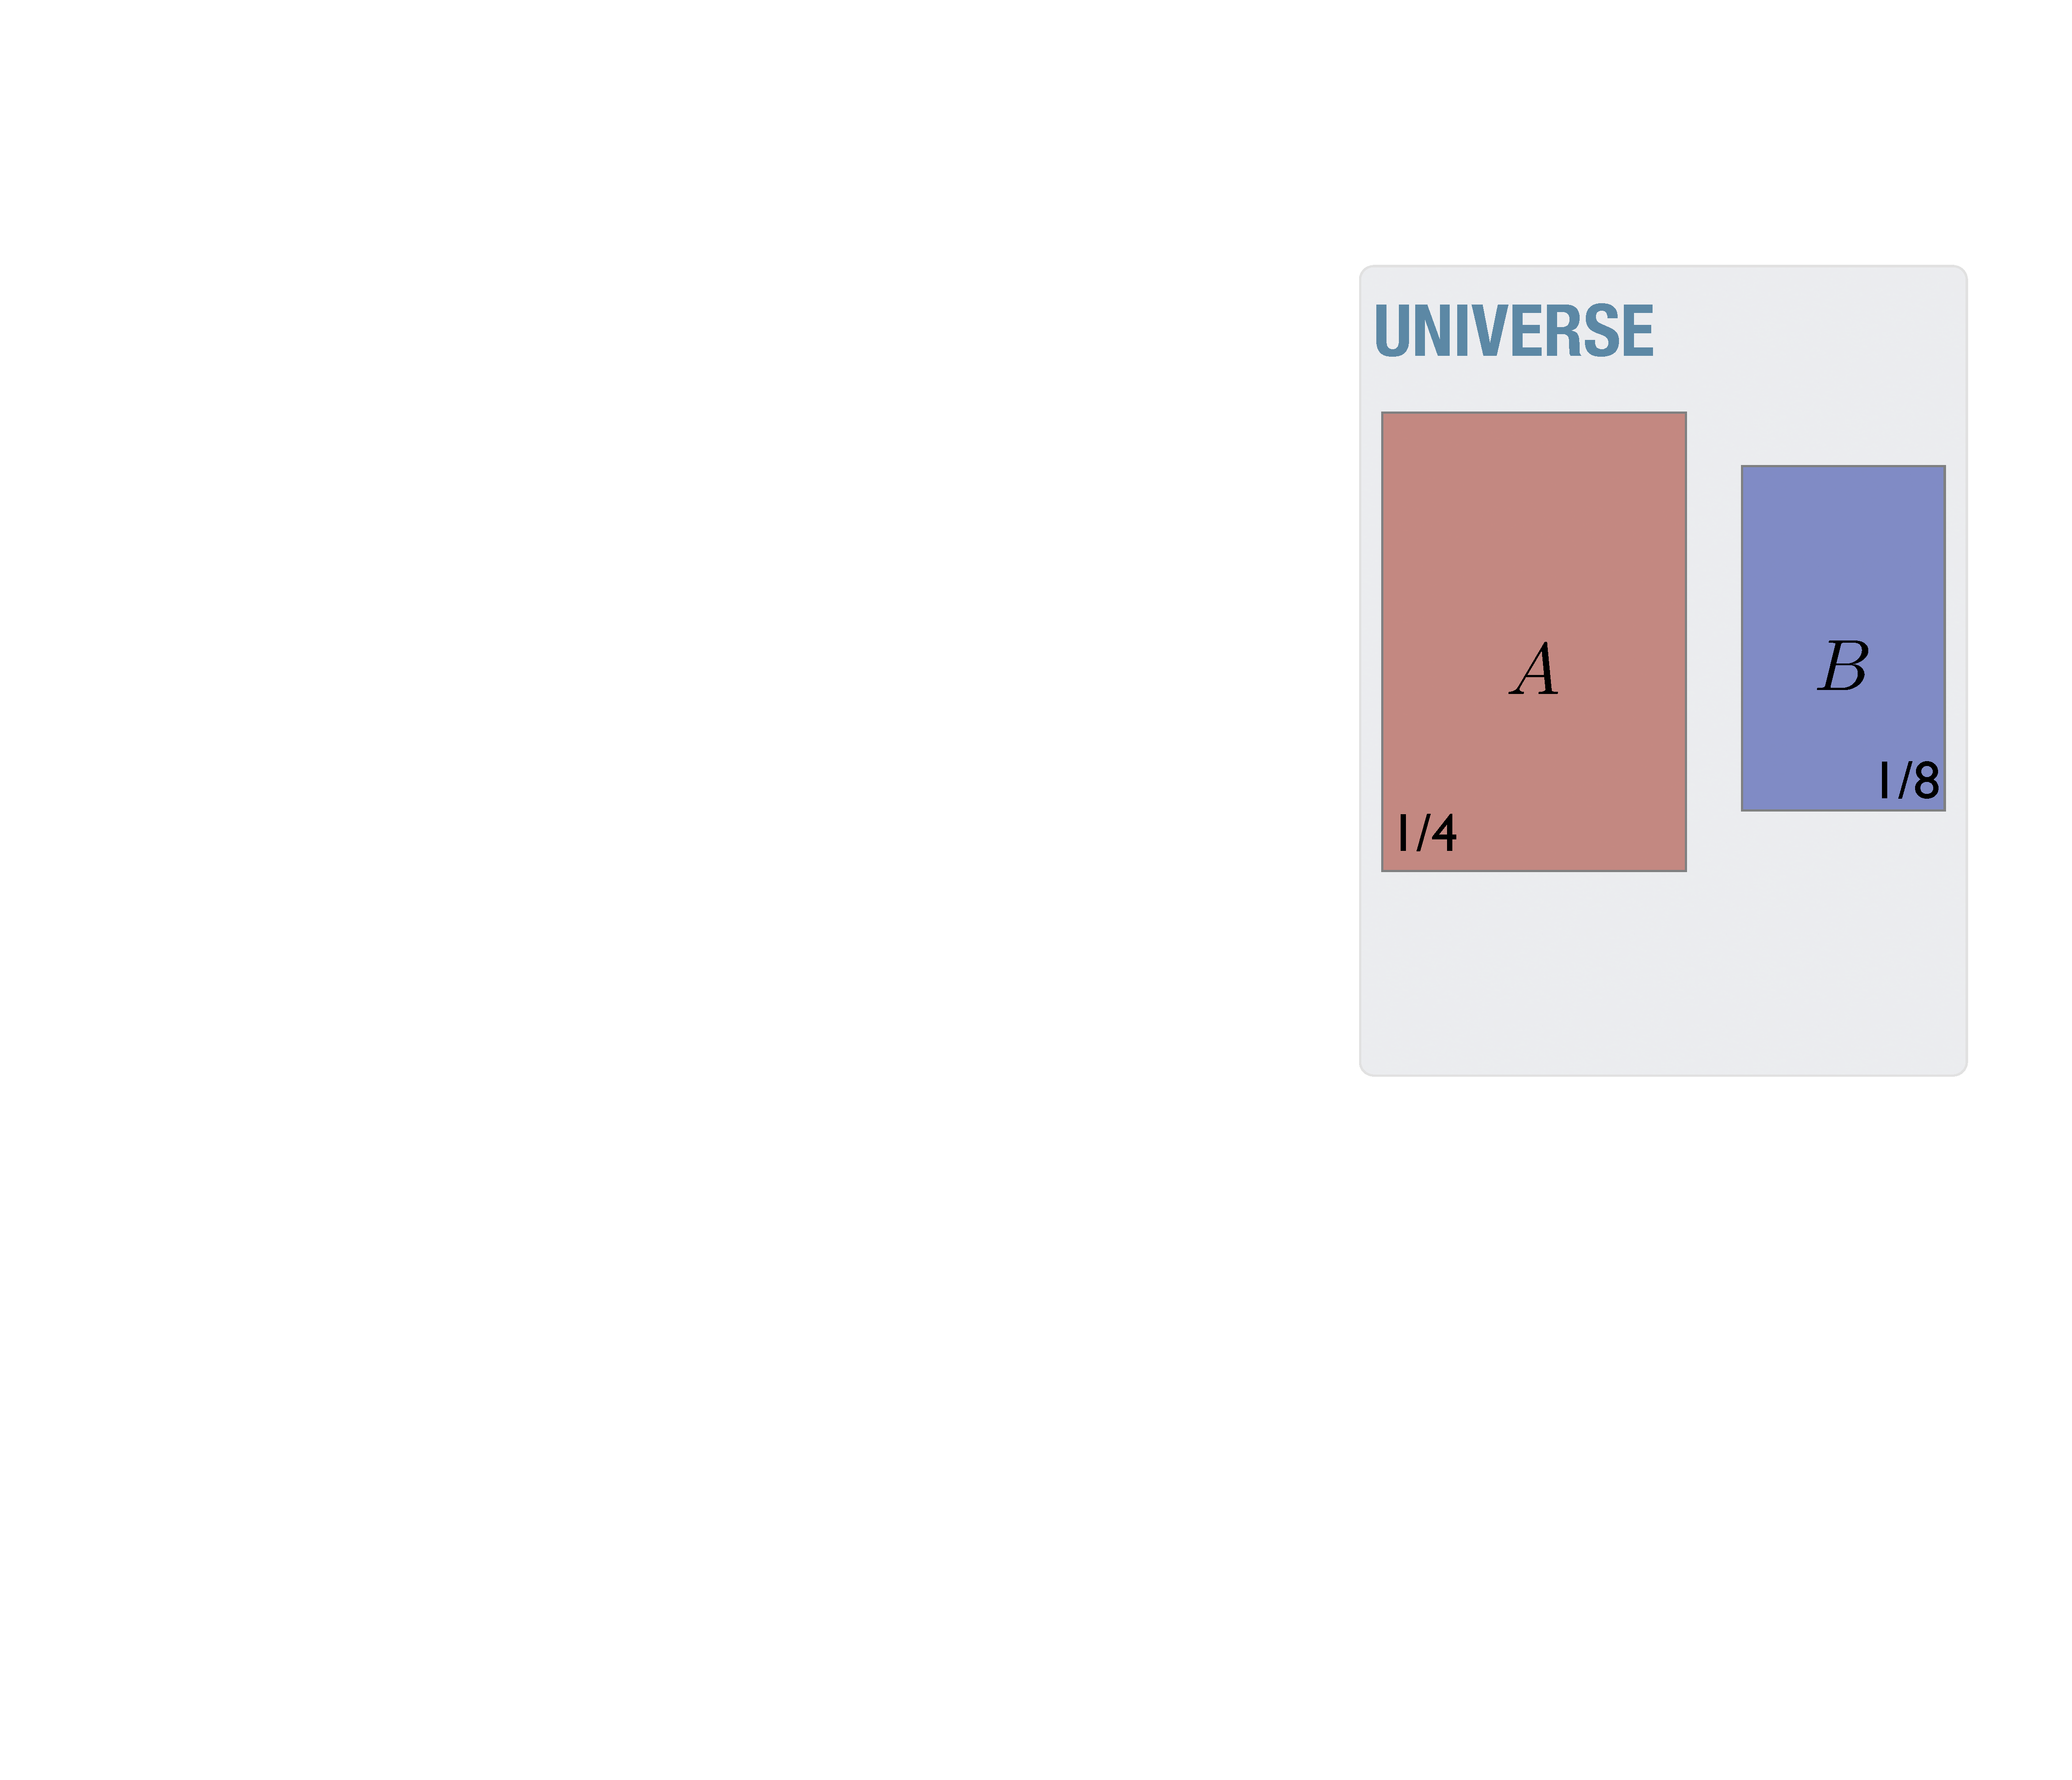
\includegraphics[width=1.4in]{venn3}
\caption{Venn diagram of mutually exclusive statements.  One can see that $P(A \mbox{ \bf and } B)=0$ (the overlap is zero) and  $P(A \mbox{ \bf or } B) = P(A)+P(B)$ (the total area is just the sum of the two areas)}
\label{fig:venn_exclusive}
\end{marginfigure}

\beqn
P(A \mbox{ \bf or } B) = P(A) + P(B)
\eeqn
Further, it is straightforward to see from this diagram the following properties for mutually exclusive events
\beqn
P(A\mbox{ \bf and } B) &=& 0 \\
P(A|B)&=&0 \\
P(B|A)&=&0
\eeqn


\section{Lessons from Bayes' Rule - A First Look}
Bayes' Rule is the gold standard for all statistical inference.  It is a mathematical theorem, proven from fundamental principles.  It structures all inference in a systematic fashion.  However, it can be used without doing any calculations, as a guide to qualitative inference.  Some of the lessons which are consequences of Bayes' Rule are listed here, and will be noted throughout this text in various examples.

\bi
\i Confidence in a claim should scale with the evidence for that claim
\i Ockham's razor, which is the philosophical idea that simpler theories are preferred, is a consequence of Bayes' Rule when comparing models of differing complexity.
\i Simpler means fewer adjustable parameters
\i Simpler also means that the predictions are both {\em specific} and not {\em overly plastic}. For example, a hypothesis which is consistent with the observed data, and also be consistent if the data were the opposite would be overly plastic.
\i Your inference is only as good as the hypotheses (i.e. models) that you consider.
\i Extraordinary claims require extraordinary evidence.\cite{sagandemon}
\i It is better to explicitly display your assumptions rather than implicitly hold them.
\i It is a {\em good thing} to update your beliefs when you receive new information.
\i Not all uncertainties are the same.
\ei


There is not a universal agreement for the translation of numerical probability values to qualitative terms in English (i.e. highly unlikely, somewhat unlikely, etc...).  One rough guide is shown in Table~\ref{table1}.  I will be following this convention throughout the book, but realize that the specific probability distinctions are a bit arbitrary.




\begin{table}
\begin{tabular}{cc}
term & probability \\\hline\hline
virtually impossible & 1/1,000,000\\
extremely unlikely & 0.01 (i.e. 1/100) \\
very unlikely & 0.05 (i.e. 1/20) \\
unlikely & 0.2 (i.e. 1/5) \\
slightly unlikely & 0.4 (i.e. 2/5) \\
even odds & 0.5 (i.e. 50-50) \\
slightly likely & 0.6 (i.e. 3/5) \\
likely & 0.8 (i.e. 4/5) \\
very likely & 0.95 (i.e. 19/20) \\
extremely likely & 0.99 (i.e. 99/100) \\
virtually certain & 999,999/1,000,000
\end{tabular}
\label{table1}
\caption{Rough guide for the conversion of qualitative labels to probability values. }
\end{table}


